\chapter{Technical Evaluation}
\label{chap:technical-evaluation}
\centerline{\rule{149mm}{.02in}}
\vspace{2cm}

We have shown that the point $kd$-tree greatly outperforms the Pyramid tree for the two scientific datasets. For all synthetic data and the 3D point cloud dataset, the Pyramid tree is faster, especially with point deletion. This chapter will explore the reasons for this, determining what properties the astrophysics dataset has which cause the performance of the structures to degenerate. The chapter will conclude by discussing the types of data suitable for the Pyramid Tree and $kd$-tree, along with some further discussion on the implications of the results from this evaluation.

\section{Characteristics of Astrophysics Dataset}
\label{sec:data-characteristics}

A dataset can be considered \textit{skewed} if there are more points in some regions of the data space than other regions. In other words, the underlying frequency or probability distribution of point locations is non-uniform. Intuitively, the skewness of a dataset increases as the \textit{difference} between the frequency, or probability, of points in different spatial regions increases.

Histograms are used to visualise the frequency distributions of one-dimensional data. Since this project deals with multi-dimensional data, multiple histograms, one for each dimension, can be produced to gain insight into point distribution. The astrophysics dataset was computed using a 3D sampling lattice, computing ten fields at each point. The original simulation uses interpolation to compute the ten fields at each point on the lattice \cite{astrophysics-dataset}. Carr et al. discusses how this interpolation ``implicitly applies the spatial relation between sample points" and shows that histograms are equivalent to nearest-neighbour interpolation \cite{histograms-and-isosurfaces}. This means histograms poorly represent datasets that use higher-order interpolants, such as the astrophysics dataset, because they ``over-emphasizes densely-sampled regions and under-emphasizes sparsely-sampled regions" \cite{histograms-and-isosurfaces}. 

Isosurface statistics have been proposed as a superior representation of such datasets \cite{histograms-and-isosurfaces}. They are conceptually and computationally more complex to compute however. Due to the project's time constraints, isosurface statistics will not be used. While histograms are poorer representation of the data, the aim of this evaluation is to get determine how large clusters of points are and determine the \textit{magnitude} of skew in the data space. Histograms still allow for this even if they are not as accurate at representing the data as other techniques. For these reason, histograms will be used to visualise the distribution of the astrophysics dataset.

\begin{figure}
	\begin{center}
		\begin{subfloat}[Dimension 1 (total particle density)]{%
			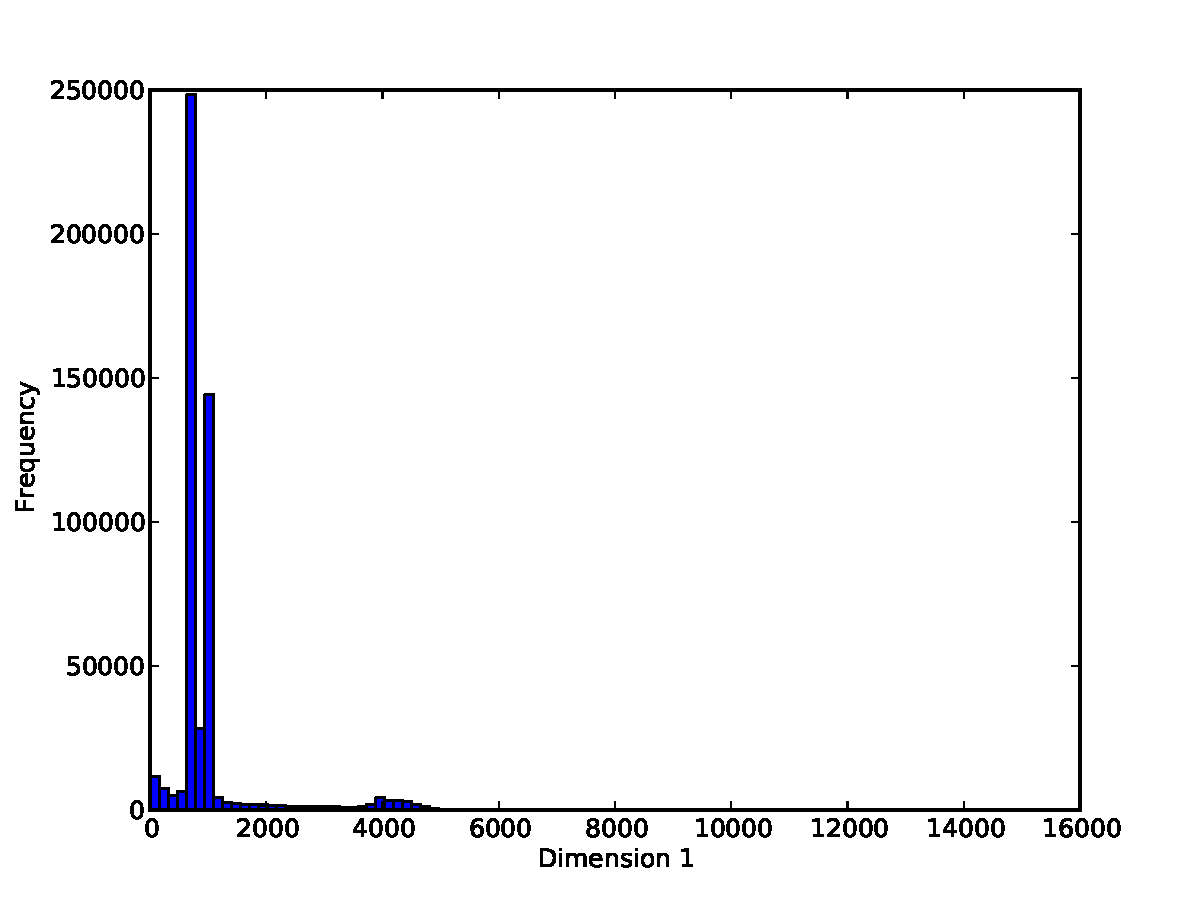
\includegraphics[scale=0.36]{figures/histograms/astrophysics_500000_0.pdf}
		}
		\end{subfloat}~
		\begin{subfloat}[Dimension 2 (gas temperature)]{%
			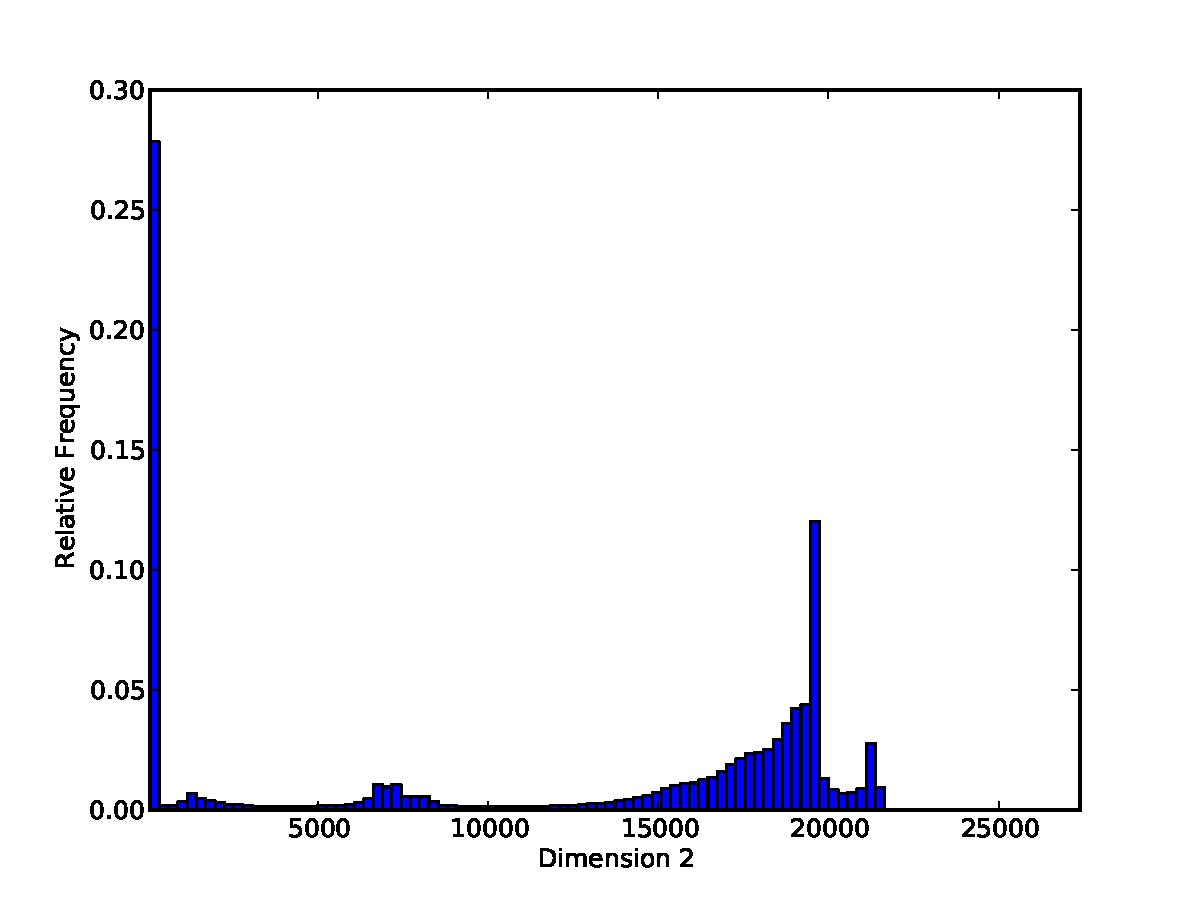
\includegraphics[scale=0.36]{figures/histograms/astrophysics_500000_1.pdf}
		}
		\end{subfloat}
	\end{center}

	\caption{Frequency Distributions of Dimensions 1 and 2 of Astrophysics Dataset}
	\label{fig:astrophysics-histograms1}
\end{figure}

\begin{figure}
	\begin{center}
		\begin{subfloat}[Dimension 3 (H mass abundance)]{%
			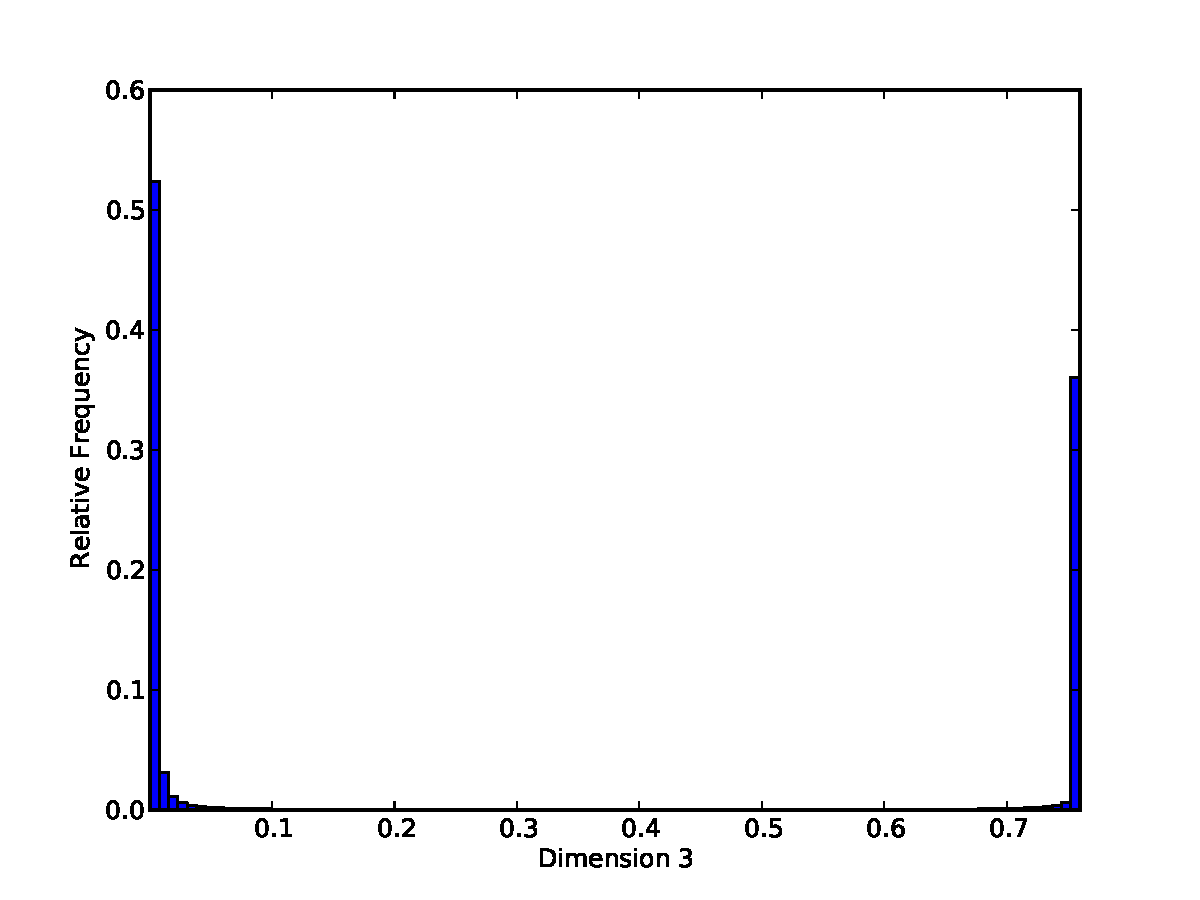
\includegraphics[scale=0.36]{figures/histograms/astrophysics_500000_2.pdf}
		}
		\end{subfloat}~
		\begin{subfloat}[Dimension 7 (He${}^{++}$ mass abundance)]{%
			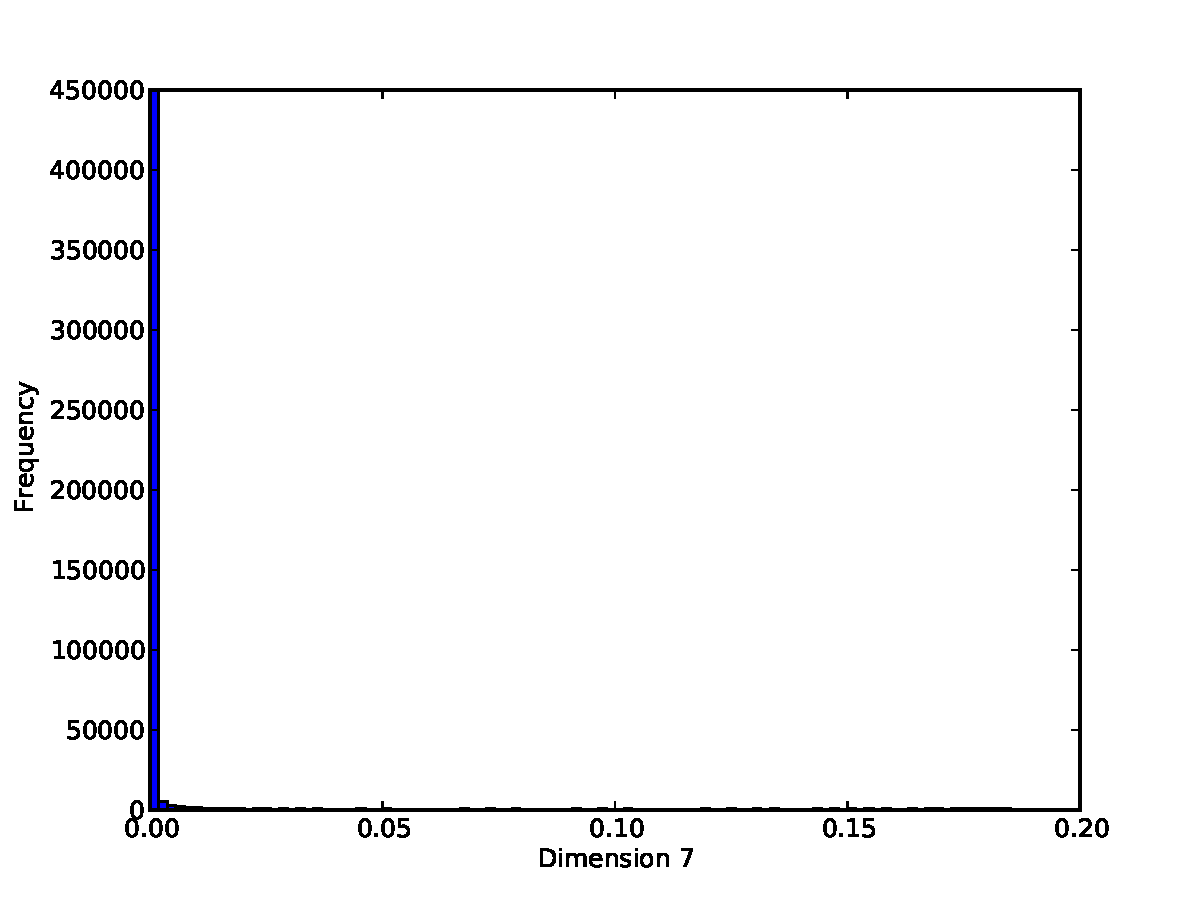
\includegraphics[scale=0.36]{figures/histograms/astrophysics_500000_6.pdf}
		}
		\end{subfloat}
	\end{center}

	\caption{Frequency Distributions of Dimensions 3 and 7 of Astrophysics Dataset}
	\label{fig:astrophysics-histograms2}
\end{figure}

Using the same sampled astrophysics dataset used for performance analysis in Chapter \ref{chap:design-and-implementation}, a histogram has been generated for each of the ten dimensions. Figures \ref{fig:astrophysics-histograms1} and \ref{fig:astrophysics-histograms2} show histograms of dimensions 1, 2, 3 and 7. The remaining dimensions have distributions similar to the dimensions shown here, so they add little value to the discussion. They can be found in Appendix \ref{sec:app-histograms} for completeness. Using these histograms, the following observations can be made:
\begin{enumerate}
	\item the first two dimensions, total particle density and gas temperature, appear to have the greatest variance, although there are still very large peaks
	\item most points are clustered on the lower or upper boundaries of dimensions 3, 4, 5 and 6. The respective histograms have massive peaks at either end of the distribution and much smaller peaks in between
	\item most points are clustered on the lower boundary of dimensions 7, 8, 9 and 10, with a single large peak on the histograms
\end{enumerate}
The astrophysics dataset is therefore highly skewed, since most points are clustered at the boundaries of each dimension. It follows that the vast majority of the data space has little to no points, making the data space \textit{sparse}.

\section{Effect of Distribution on Pyramid Tree}

We now explore the effect of the highly skewed distribution on the Pyramid Tree. Recall that the Pyramid Tree maps a point $v$ to a single scalar named the Pyramid value $pv_v$. Points with the same Pyramid value are stored in the same bucket. Table \ref{tab:final-bucket-size} shows bucket size statistics and how long it takes to query all the points for the sampled astrophysics dataset with different subsets of dimensions. When only dimensions 1 and 2, the dimensions with the greatest variance, are used, average bucket size decreases substantially. Dimensions 3 and 7 have larger clusters of points close together, so they cause the average bucket size to increase.

The histograms from Section \ref{sec:data-characteristics} illustrate how most points lie on, or close to, the boundaries of the dataset. This is a significant problem for the Pyramid Tree because it always chooses the dimension whose distance from the centre point of the data is the highest. If a large number of points are on a dimensional boundary, then its likely the same dimension will be chosen. Each point will the same coordinate value for the chosen dimension because they are on the same boundary, meaning will have the same pyramid value and will be mapped to the same bucket.

\begin{table}
	\centering
	\makebox[\textwidth][c]{%
		\begin{tabular}{|l|l|l|l|l|}
			\hline
			\textbf{Dimensions} & \textbf{Time to Query (sec)} & \textbf{Average} & \textbf{Max} & \textbf{\#Buckets} \\
			\hline
			All & 60.0216 & 3586.57 & 235260 & 120 \\
			1 and 2 & 0.0713558 & 6.52433 & 102 & 25232 \\
			3 and 7 & 8.30587 & 89.2853 & 141235 & 3056 \\
			\hline
			No Boundary Coordinates & 27.6034 & 25.3722 & 45031 & 16963 \\
			\hline
		\end{tabular}
	}%
	\caption{Pyramid Tree Bucket Size Statistics with Different Dimensions of Astrophysics Dataset}
	\label{tab:final-bucket-size}
\end{table}

Histograms are equivalent to nearest-neighbour interpolation, so they do not show if the points inside the bins at the boundary of the graphs are \textit{actually} boundary values or just close to the boundary. To determine if clusters of points at boundaries is truly the main cause of large buckets, a heuristic called \textbf{No Boundary Coordinates} was developed. Let $v$ be a point and $min_i$ and $max_i$ be the minimum and maximum boundary values for dimension $i \in \lbrace 0, 1, ..., d - 1 \rbrace$. Let $j$ be the dimension $v$ is furthest away from the centre point with. If $v_j = min_j$ or $v_j = max_j$, then a new dimension $k$ is chosen, such that $v_k$ is the \textit{second} furthest coordinate from the centre point. If $v_k$ is at the boundary, then the next furthest is chosen. This process is repeated until a coordinate which is not on a boundary is found. If all coordinates are on a boundary, then the first dimension is chosen.

Table \ref{tab:final-bucket-size} shows how this simple heuristic decreases average bucket size. However, it is still significantly slower than the $kd$-tree, so other kinds of skew are still causing problems. One could apply further heuristics in an attempt to improve Pyramid Tree performance on the astrophysics dataset, but it is likely that the structure will start overfitting the dataset and performing worse on other datasets. Creating heurstics like this requires pre-existing knowledge of the dataset's distribution, which may not be available, especially when the data dynamic (i.e. it is not \textit{possible} to know all the data in advance).

\section{Effect of Distribution on $kd$-tree}

For completeness, different dimensions of the astrophysics dataset were also tested on the point $kd$-tree. Table \ref{tab:final-balance-factor} shows the query time, balance factor and maximum path length of the tree with these different dimensions. It can be observed that the point $kd$-tree, like the Pyramid Tree, performs worse because of the skew present in the astrophysics dataset as well. Using dimensions 1 and 2 gives a lower balance factor than the more skewed dimensions 3 and 7. The difference in performance between the chosen dimensions is much smaller than the Pyramid tree, however, again showing the point $kd$-tree is more resilient to skew.

\begin{table}
	\centering
	\makebox[\textwidth][c]{%
		\begin{tabular}{|l|l|l|l|l|}
			\hline
			\textbf{Dimensions} & \textbf{Time to Query (sec)}  & \textbf{Balance Factor} & \textbf{Max Path Length}  \\
			\hline
			All & 0.639265 & 32.405 & 120 \\
			1 and 2 & 0.18445 & 26.5923 & 73 \\
			3 and 7 & 0.257211 & 28.6481 & 69 \\
			\hline
		\end{tabular}
	}%
	\caption{Point $kd$-tree Statistics with Different Dimensions of Astrophysics Dataset}
	\label{tab:final-balance-factor}
\end{table}

\section{Conjecture on Scientific Datasets}

While an analysis of the hurricane Isabel dataset is not in this report, generating histograms of each dimension reveals distributions similar to the astrophysics dataset. Some dimensions have smoother distributions, whereas others contain large clusters of points at the boundaries. This raises an important question: do datasets resulting from scientific simulations generally have these properties, or are these properties just specific to these datasets? If the former is true, more general hypotheses can be made regarding the index structures that are suitable for scientific computation and visualisation.

Exploring the properties of scientific multi-dimensional datasets is a project in itself, so an in-depth analysis of such properties will not be performed. Instead, existing literature will be used as the basis for the following conjecture.

\paragraph{\textbf{CONJECTURE:}} Dense clusters of points and large sparse regions of data space is a property present in the majority of scientific datasets computed using sampling lattices. 
\paragraph{}

Scientific datasets are often computed using $m$-dimensional sampling lattices, where each point on the lattice represents a point in physical space, as was the case with the astrophysics dataset \cite{astrophysics-dataset}. This means $m$ is usually 2 or 3. $d$ continuous fields are measured at each point, which are typically physical properties such as temperature, wind velocity, chemical masses and so on. Interpolation is applied in some way to model the spatial relationships between the properties of the sampling points in physical space.

Often, $d > m$, like with the astrophysics and hurricane Isabel datasets. Such physical simulations can be described as a mapping $\mathbb{R}^m \rightarrow \mathbb{R}^d$, where $d > m$. As $d$ increases, the resulting data space's volume increases exponentially, resulting in sparsity (as discussed in Section \ref{sec:curse-of-dimensionality}). To fill the data space, an exponentially increasing number of data points must be sampled, which is not viable for high $d$.

Data sparsity becomes an even greater issue when mapping continuous domains to higher dimensional space because the resulting $d$-dimensional dataset becomes a sampled $m$-dimensional manifold in $d$-dimensional space. Figure \ref{fig:manifolds} illustrates examples of manifolds for $\mathbb{R}^1 \rightarrow \mathbb{R}^2$ and $\mathbb{R}^2 \rightarrow \mathbb{R}^3$. Notice how the majority of the data spaces are empty in both examples. Only thin strips of the data spaces are filled by the lower-dimensional manifolds. The astrophysics dataset was the result of a $\mathbb{R}^3 \rightarrow \mathbb{R}^{10}$ simulation, so a 3 dimensional manifold is embedded in 10 dimensional space. This results in a highly sparse space, which may be one of the reasons there are so many large clusters of points in the astrophysics dataset.

\begin{figure}
	\begin{center}
		\begin{subfloat}[$\mathbb{R}^1 \rightarrow \mathbb{R}^2$]{%
			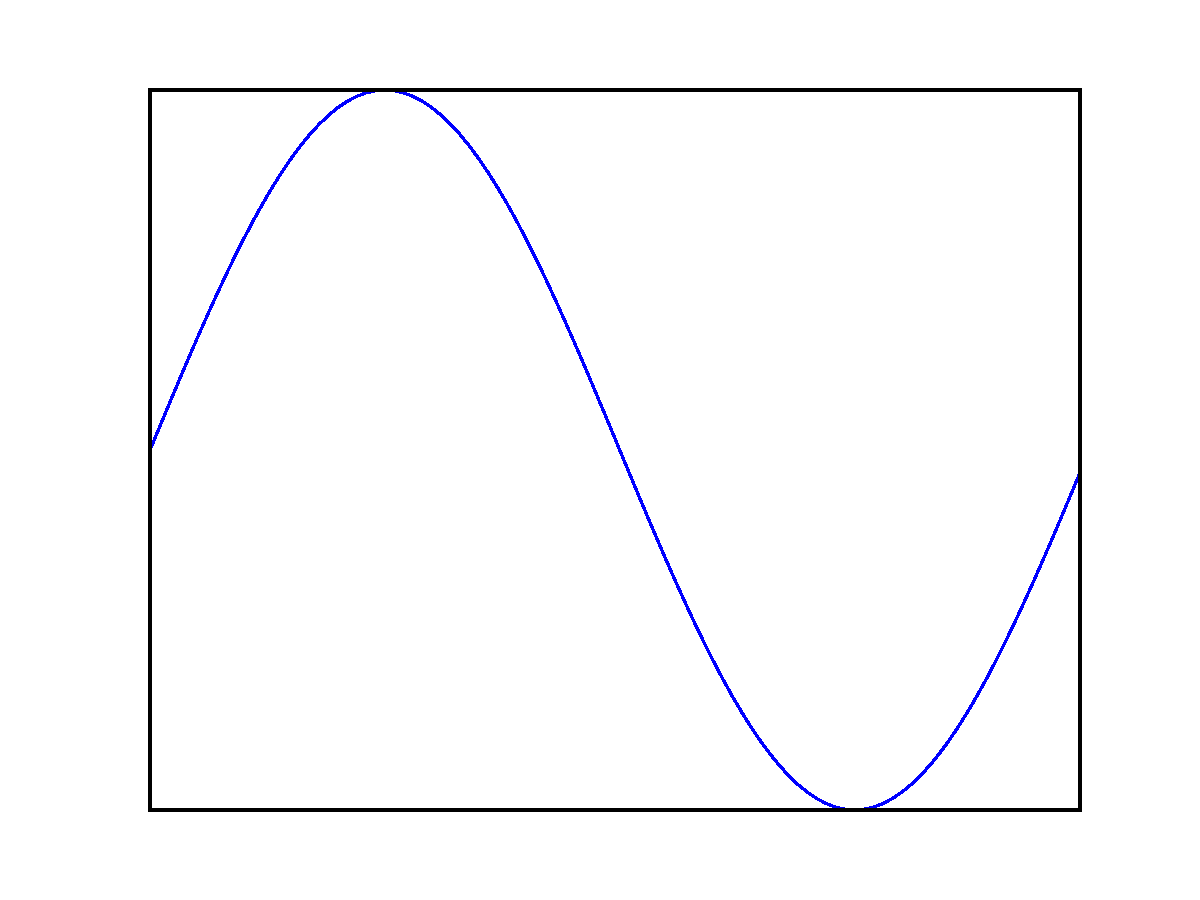
\includegraphics[scale=0.2]{figures/1d_manifold.pdf}
		}
		\end{subfloat}~
		\begin{subfloat}[$\mathbb{R}^2 \rightarrow \mathbb{R}^3$]{%
			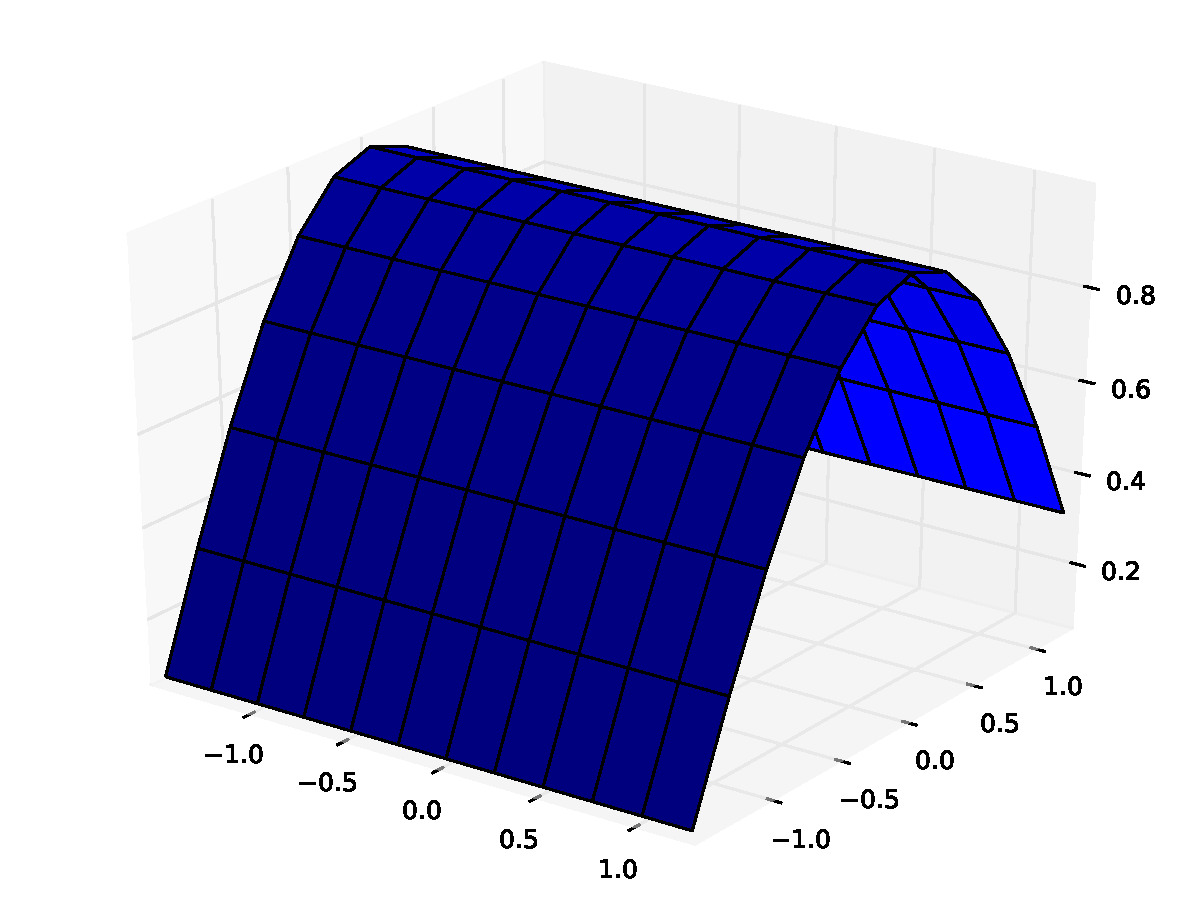
\includegraphics[scale=0.225]{figures/2d_manifold.pdf}
		}
		\end{subfloat}
	\end{center}

	\caption{Manifolds Embedded in Higher-Dimensional Space}
	\label{fig:manifolds}
\end{figure}

\section{Implications to Multi-dimensional Search}

This conjecture has implications for which index structures to use for scientific datasets. If most scientific datasets are highly space, they may be difficult for index structures which decompose the underlying data space. For example, the Pyramid Tree uses a \textit{static} decomposition. Based on an initial boundary, exactly how the space is decomposed is already decided. For some data, such as the synthetic data used in Chapter \ref{chap:design-and-implementation}, this is not a problem. However, there cases where the lack of ability to \textit{adapt} the decomposition to the input data becomes problematic. This was the case with the astrophysics dataset, where the Pyramid Tree ended up mapping the points to the same few buckets.

\begin{figure}
	\begin{center}
		\begin{subfloat}[Non-Continuous Embedding Decomposed with Pyramid Tree\label{fig:non-continuous-embedding}]{%
			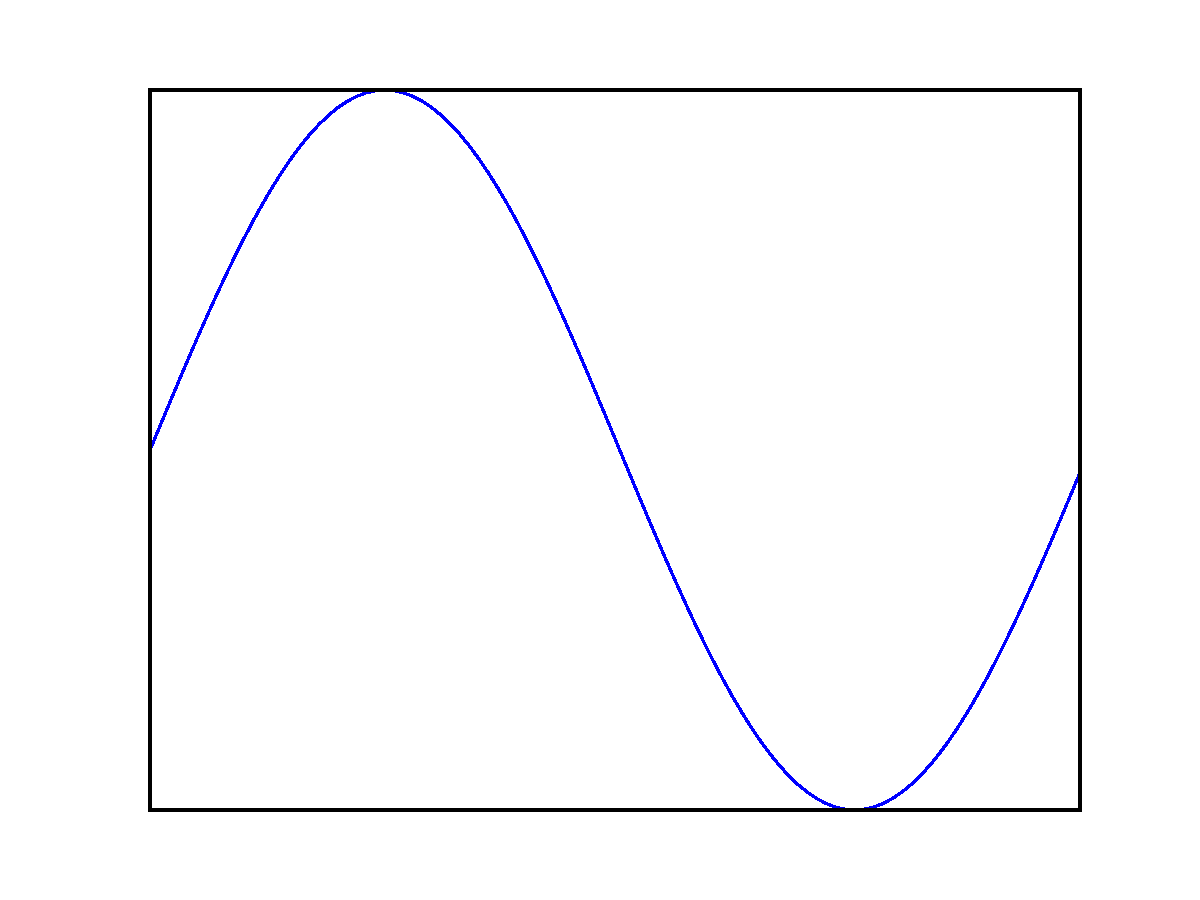
\includegraphics[scale=0.2]{figures/1d_manifold.pdf}%{figures/non-continuous-pyramid.pdf}
		}
		\end{subfloat}~
		\begin{subfloat}[Continuous Embedding Decomposed with Pyramid Tree\label{fig:continuous-embedding-pyramid}]{%
			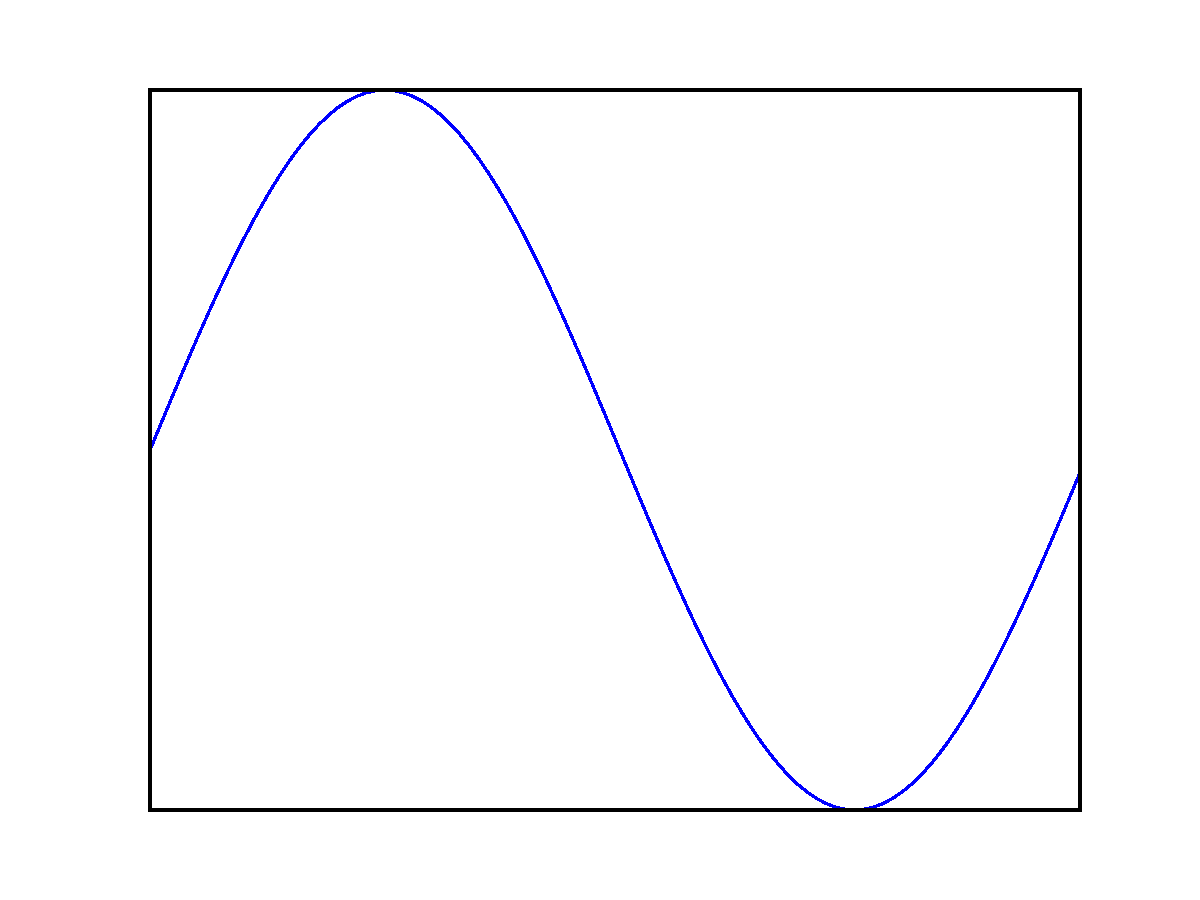
\includegraphics[scale=0.2]{figures/1d_manifold.pdf}%{figures/continuous-pyramid.pdf}
		}
		\end{subfloat}~
		\begin{subfloat}[Continuous Embedding Decomposed with Adaptive Octree\label{fig:continuous-embedding-octree}]{%
			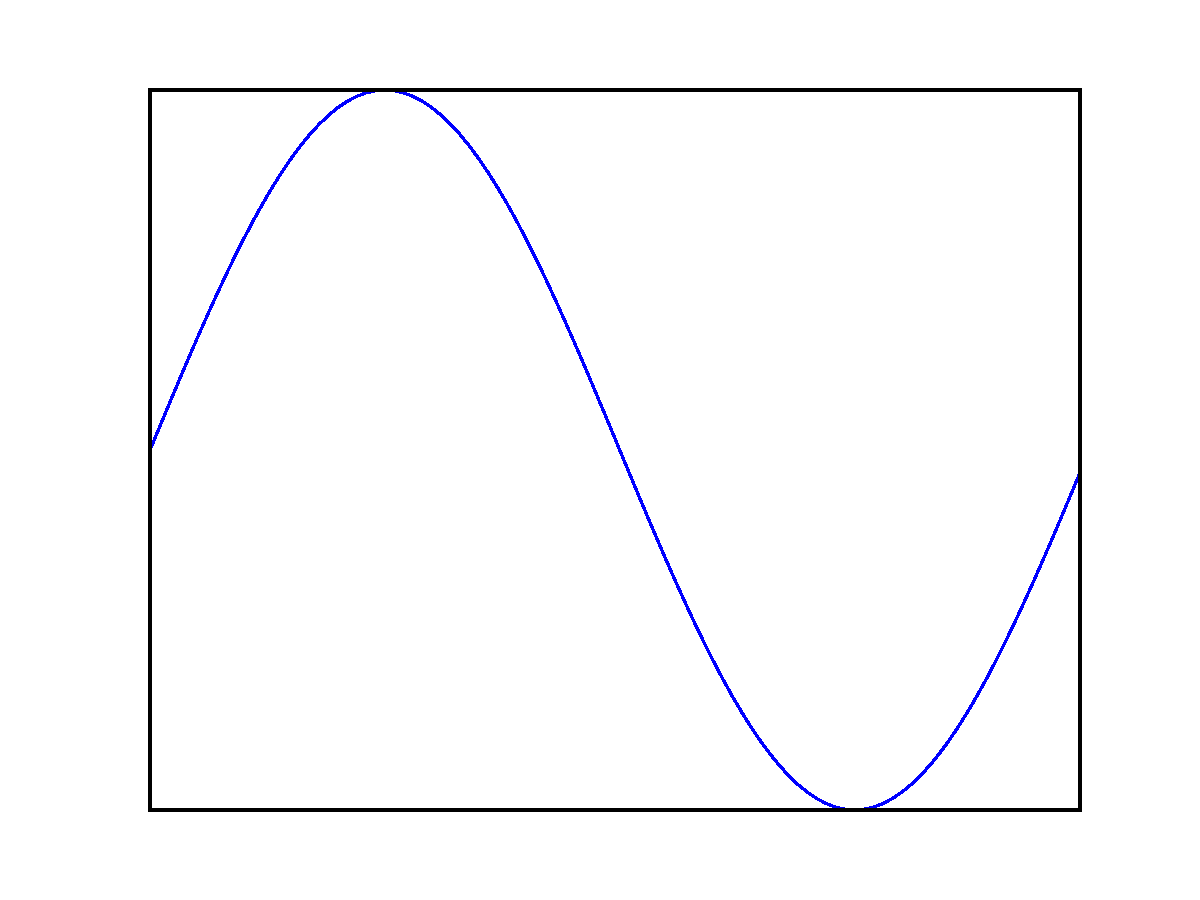
\includegraphics[scale=0.2]{figures/1d_manifold.pdf}%{figures/continuous-pyramid.pdf}
		}
		\end{subfloat}
	\end{center}

	\caption{Static and Adaptive Decomposition of Datasets}
	\label{fig:static-adaptive-decomposition}
\end{figure}

Figure \ref{fig:non-continuous-embedding} shows a dataset computed using the mapping $f : \mathbb{R}^1 \rightarrow \mathbb{R}^2$. Unlike the astrophysics dataset, $f$ is not modelling continuous physical phenomenon and a such, the resulting dataset in $\mathbb{R}^2$ is not continuous (i.e. is not a curve). This would be the case for the synthetic data randomly generated for performance analysis previously. In this particular example,. 

Figure \ref{fig:continuous-embedding-pyramid} shows a continuous one-dimensional manifold. It is similar to the astrophysics dataset in that strips of points are aligned along some value close to the boundary. The Pyramid Tree ends up storing all the points in just threes buckets. Without the ability to adapt, the performance of the structure will rapidly degrade as more and more points are mapped to the same few buckets. Recall that the original Pyramid Tree paper evaluated the structure using a discrete text database and range queries \cite{pyramid-tree}. Continuous data with point queries was not tested, so it is not entirely surprising that the Pyramid Tree's performance is poor.

Figure \ref{fig:continuous-embedding-octree} shows an adaptive Octree decomposition, which adapts the decomposition by providing greater discrimination between points in regions that contain more points. The point $kd$-tree can be seen as an adaptive index structure to some extent, since decomposition of the underlying data space depends on the values of the given points. This, along with its resilience to points aligned in strips close to boundaries, are some of the reasons its performance is vastly superior to the Pyramid Tree for the two scientific datasets.

\section{Suitability of Hash-Based Approaches}

The Pseudo-Pyramid Tree and Pyramid Tree both produce a static decomposition of the underlying data space through the use of dimension reduction (i.e. they \textit{hash} points). They do not adapt to the distribution of the input data by modifying the amount or size of bins. With dynamic data, where one does not know the distribution of the data in advance, these approaches are severely limited. This is shown by the empirical results from this project; the performance of these two structures on the real datasets is vastly inferior to the point $kd$-tree, a simple and well-established technique.

Adaptive variants of the Pyramid Tree exist, such as the Extended Pyramid-Technique \cite{pyramid-tree} and IMinMax($\theta$) \cite{iminmax}. However, the \textit{cost} of adapting such structures limits their usefulness. For example, the Extended Pyramid-Technique moves the centre of the data space to be the median point. Doing so means that the entire structure must be rebuild, because each stored point may be hashed to a different value after the data space is moved. For large $n$ this has a massive impact on performance. Suppose the structure stores a million points and then has to adapt -- a million points must be re-inserted. IMinMax($\theta$) was implemented in this project, but the performance was still poor despite it adapting to the dataset, due of the rebuilding procedure. For this reason, it has not been covered in detail in this report and the project did not explore adaptive dimension reduction techniques any further.

Despite the more adaptive point $kd$-tree performing worse on highly skewed data like the astrophysics dataset, the structure can still process the data reasonably quickly. No major optimisations were applied to the implementation and no additional exploration was performed the numerous $kd$-tree variants that have been developed.

The empirical performance timings has lead the author of this report to conclude that techniques which perform a static decomposition of the data space are \textit{not} suitable for dynamic data, unless one knows about the kinds of distributions that will be given in advance. The supplementary theoretical analysis performed in this chapter has shown that data generated by mapping continuous domains mapped to higher-dimensional ranges are especially a challenge for structures that cannot adapt, due to the highly clustered and skewed distributions of points that result from such a mapping. Since the cost of adapting dimension reduction technique is so high due to rebuilds being required, perhaps dimension reduction in general is not suitable for dynamic data.

Index structures which can adapt to different distributions of data \textit{as} points are inserted tend to require less computation. From initial experimentation with the point $kd$-tree, they appear to offer good performance with point queries. The literature often discussed how $kd$-trees degenerate to Sequential Scan with higher dimensions, but this does not appear to be the case for point queries.

\section{New Hypotheses}

Based on the empirical evidence from Chapter \ref{chap:design-and-implementation} and the theoretical evaluation from Chapter \ref{chap:technical-evaluation}, the hypothesis from Section \ref{sec:main-hypothesis} has been abandoned in favour of the following new hypothesis.

\paragraph{\textbf{HYPOTHESIS 1:}} The Pyramid Tree is not a suitable index structure for performing point queries in higher-dimensional scientific datasets.

\paragraph{\textbf{HYPOTHESIS 2:}} Index structures based on dimension reduction or hashing cannot adapt well to dynamically changing distributions of data, due to the cost of rebuilding the structure when adapting.

\paragraph{\textbf{HYPOTHESIS 3:}} Dynamic tree-based structures, which adapt the decomposition of the data space as points are inserted, provide better point query performance for dynamic high-dimensional datasets than dimension reduction techniques such as the Pyramid Tree.

\paragraph{}

Hypothesis 1 has been verified specifically for the astrophysics (and to a lesser extent, the hurricane Isabel dataset). More research and analysis with other scientific datasets is required to fully verify both this hypotheses. Some evidence verifying hypotheses 2 and 3 is present in this report, as there are empirical timings to support the clams, but more comprehensive research should be performed. it is beyond the scope of this project to explore these hypotheses further, however.